\documentclass[t,usenames,dvipsnames]{beamer}
\usetheme{Copenhagen}
\setbeamertemplate{headline}{} % remove toc from headers
\beamertemplatenavigationsymbolsempty

\usepackage{amsmath, tikz, xcolor, bm, pgfplots}
\pgfplotsset{compat = newest}
\usetikzlibrary{arrows, calc, decorations.pathreplacing, patterns}

\title{Hyperbolas}
\author{}
\date{}

\AtBeginSection[]
{
  \begin{frame}
    \frametitle{Objectives}
    \tableofcontents[currentsection]
  \end{frame}
}

\begin{document}

\begin{frame}
    \titlepage
\end{frame}

\begin{frame}{Intro}
The definition of a hyperbola is the same as the definition of an ellipse. The only difference is we replace the word \emph{sum} in the definition of an ellipse with \emph{difference} for a hyperbola.  \newline\\  \pause

A \alert{hyperbola} is the set of points such that the \underline{difference} of their distances from 2 fixed points (called \alert{foci}) is constant.
\end{frame}

\begin{frame}{Intro}
Just like an ellipse, the midpoint joining the foci is the \textbf{center}.    \newline\\   \pause

Whereas ellipses could appear taller or wider, hyperbolas will open up and down, or left and right. \newline\\  \pause

A key difference, however, is that hyperbolas will open left/right if the sign in front of $x$ is positive, and will open up/down if the sign in front of $y$ is positive; regardless of the values of $a$ and $b$.  
\end{frame}

\begin{frame}{Intro}
\begin{center}
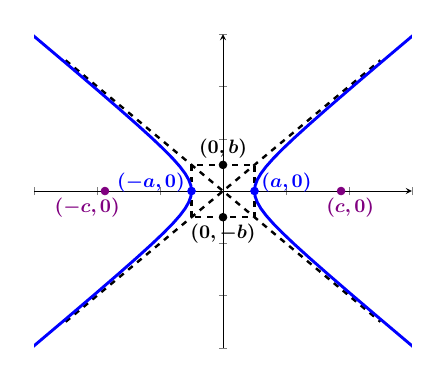
\begin{tikzpicture}[scale=0.7]
\begin{axis}[
axis lines = middle,
%grid,
xticklabels = {},
yticklabels = {},
xmin = -6, xmax = 6,
ymin = -6, ymax = 6
]
\draw [dashed, line width=1.25] (-1,-1) rectangle (1,1);
\draw [dashed, line width=1.25] (-5,-5) -- (5,5);
\draw [dashed, line width=1.25] (-5,5) -- (5,-5);
\addplot [blue, line width = 1.5, domain=-2.5:2.5] ({cosh(x)}, {sinh(x)});
\addplot [blue, line width = 1.5, domain=-2.5:2.5] (-{cosh(x)}, {sinh(x)});
\draw [fill=blue, color=blue] (-1,0) circle (2pt);
\node at (-1,0) [anchor=south east, color=blue, yshift=-0.15cm] {$\bm{(-a,0)}$};
\draw [fill=blue, color=blue] (1,0) circle (2pt);
\node at (1,0) [anchor=south west, color=blue, yshift=-0.15cm] {$\bm{(a,0)}$};
\draw [fill=violet, color=violet] (3.75,0) circle (2pt);
\node at (3.5,0) [anchor=north west, color=violet, xshift=-0.25cm] {$\bm{(c,0)}$};
\draw [fill=violet, color=violet] (-3.75,0) circle (2pt);
\node at (-3.5,0) [anchor=north east, color=violet, xshift=0.25cm] {$\bm{(-c,0)}$};
\draw [fill=black] (0,1) circle (2pt);
\node at (0,1) [anchor=south] {$\bm{(0,b)}$};
\draw [fill=black] (0,-1) circle (2pt);
\node at (0,-1) [anchor=north] {$\bm{(0,-b)}$};
\end{axis}
\end{tikzpicture} \newline\\
\begin{tabular}{rl}
    \onslide<2->{\textbf{Equation}  &    $\dfrac{(x-h)^2}{a^2} - \dfrac{(y-k)^2}{b^2} = 1$\\[10pt]}   
    \onslide<3->{\textbf{Vertices}   &   $(h\pm a,k)$\\[10pt]} 
    \onslide<4->{\textbf{Foci}   &   $(h\pm c,k)$ \\} 
\end{tabular}
\end{center}
\end{frame}

\begin{frame}{Intro}
\begin{center}
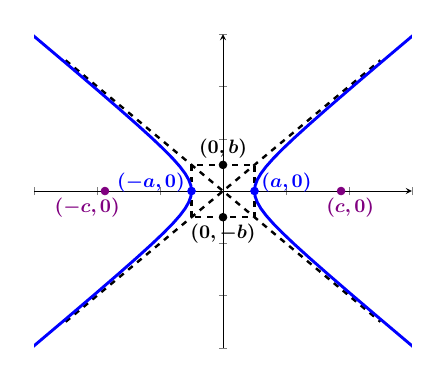
\begin{tikzpicture}[scale=0.7]
\begin{axis}[
axis lines = middle,
%grid,
xticklabels = {},
yticklabels = {},
xmin = -6, xmax = 6,
ymin = -6, ymax = 6
]
\draw [dashed, line width=1.25] (-1,-1) rectangle (1,1);
\draw [dashed, line width=1.25] (-5,-5) -- (5,5);
\draw [dashed, line width=1.25] (-5,5) -- (5,-5);
\addplot [blue, line width = 1.5, domain=-2.5:2.5] ({cosh(x)}, {sinh(x)});
\addplot [blue, line width = 1.5, domain=-2.5:2.5] (-{cosh(x)}, {sinh(x)});
\draw [fill=blue, color=blue] (-1,0) circle (2pt);
\node at (-1,0) [anchor=south east, color=blue, yshift=-0.15cm] {$\bm{(-a,0)}$};
\draw [fill=blue, color=blue] (1,0) circle (2pt);
\node at (1,0) [anchor=south west, color=blue, yshift=-0.15cm] {$\bm{(a,0)}$};
\draw [fill=violet, color=violet] (3.75,0) circle (2pt);
\node at (3.5,0) [anchor=north west, color=violet, xshift=-0.25cm] {$\bm{(c,0)}$};
\draw [fill=violet, color=violet] (-3.75,0) circle (2pt);
\node at (-3.5,0) [anchor=north east, color=violet, xshift=0.25cm] {$\bm{(-c,0)}$};
\draw [fill=black] (0,1) circle (2pt);
\node at (0,1) [anchor=south] {$\bm{(0,b)}$};
\draw [fill=black] (0,-1) circle (2pt);
\node at (0,-1) [anchor=north] {$\bm{(0,-b)}$};
\end{axis}
\end{tikzpicture}   \newline\\
\begin{tabular}{rl}
    \onslide<2->{\textbf{\textit{x}-Axis}    &   Traverse Axis\\[10pt]}   
    \onslide<3->{\textbf{\textit{y}-Axis}    &   Conjugate Axis  \\}   
\end{tabular}
\end{center}
\end{frame}

\begin{frame}{Intro}
\begin{center}
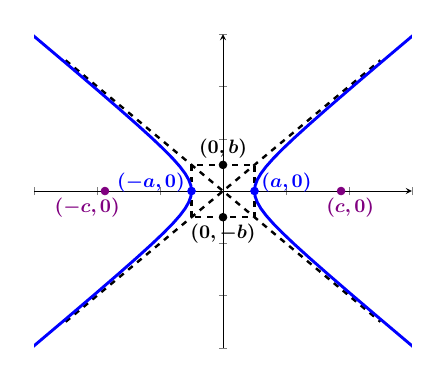
\begin{tikzpicture}[scale=0.7]
\begin{axis}[
axis lines = middle,
%grid,
xticklabels = {},
yticklabels = {},
xmin = -6, xmax = 6,
ymin = -6, ymax = 6
]
\draw [dashed, line width=1.25] (-1,-1) rectangle (1,1);
\draw [dashed, line width=1.25] (-5,-5) -- (5,5);
\draw [dashed, line width=1.25] (-5,5) -- (5,-5);
\addplot [blue, line width = 1.5, domain=-2.5:2.5] ({cosh(x)}, {sinh(x)});
\addplot [blue, line width = 1.5, domain=-2.5:2.5] (-{cosh(x)}, {sinh(x)});
\draw [fill=blue, color=blue] (-1,0) circle (2pt);
\node at (-1,0) [anchor=south east, color=blue, yshift=-0.15cm] {$\bm{(-a,0)}$};
\draw [fill=blue, color=blue] (1,0) circle (2pt);
\node at (1,0) [anchor=south west, color=blue, yshift=-0.15cm] {$\bm{(a,0)}$};
\draw [fill=violet, color=violet] (3.75,0) circle (2pt);
\node at (3.5,0) [anchor=north west, color=violet, xshift=-0.25cm] {$\bm{(c,0)}$};
\draw [fill=violet, color=violet] (-3.75,0) circle (2pt);
\node at (-3.5,0) [anchor=north east, color=violet, xshift=0.25cm] {$\bm{(-c,0)}$};
\draw [fill=black] (0,1) circle (2pt);
\node at (0,1) [anchor=south] {$\bm{(0,b)}$};
\draw [fill=black] (0,-1) circle (2pt);
\node at (0,-1) [anchor=north] {$\bm{(0,-b)}$};
\end{axis}
\end{tikzpicture}   \newline\\
\begin{tabular}{rl}
    \onslide<2->{$\bm{c^2}$  &   $=a^2+b^2$\\[10pt]}   
    \onslide<3->{\textbf{Asymptotes} &   $y = \pm \dfrac{b}{a}(x-h) + k$  \\}  
\end{tabular}
\end{center}
\end{frame}

\begin{frame}{Intro}
\begin{center}
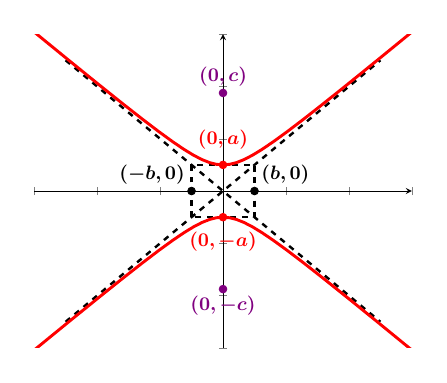
\begin{tikzpicture}[scale=0.7]
\begin{axis}[
axis lines = middle,
%grid,
xticklabels = {},
yticklabels = {},
xmin = -6, xmax = 6,
ymin = -6, ymax = 6
]
\draw [dashed, line width=1.25] (-1,-1) rectangle (1,1);
\draw [dashed, line width=1.25] (-5,-5) -- (5,5);
\draw [dashed, line width=1.25] (-5,5) -- (5,-5);
\addplot [red, line width = 1.5, domain=-2.5:2.5] ({sinh(x)}, {cosh(x)});
\addplot [red, line width = 1.5, domain=-2.5:2.5] ({sinh(x)}, {-cosh(x)});
\draw [fill=red, color=red] (0,1) circle (2pt);
\node at (0,1) [anchor=south, color=red, yshift=0.15cm] {$\bm{(0,a)}$};
\draw [fill=blue, color=red] (0,-1) circle (2pt);
\node at (0,-1) [anchor=north, color=red, yshift=-0.15cm] {$\bm{(0,-a)}$};
\draw [fill=violet, color=violet] (0,3.75) circle (2pt);
\node at (0,3.75) [anchor=south, color=violet] {$\bm{(0,c)}$};
\draw [fill=violet, color=violet] (0,-3.75) circle (2pt);
\node at (0,-3.75) [anchor=north, color=violet] {$\bm{(0,-c)}$};
\draw [fill=black] (1,0) circle (2pt);
\node at (1,0) [anchor=south west] {$\bm{(b,0)}$};
\draw [fill=black] (-1,0) circle (2pt);
\node at (-1,0) [anchor=south east] {$\bm{(-b,0)}$};
\end{axis}
\end{tikzpicture}   \newline\\
\begin{tabular}{rl}
    \onslide<2->{\textbf{Equation}  &     $\dfrac{(y-k)^2}{a^2} - \dfrac{(x-h)^2}{b^2} = 1$}   \\[0.2in]
    \onslide<3->{\textbf{Vertices}   &      $(h,k\pm a)$} \\[0.15in]
    \onslide<4->{\textbf{Foci}    &   $(h, k\pm c)$}    \\
\end{tabular}
\end{center}
\end{frame}

\begin{frame}{Intro}
\begin{center}
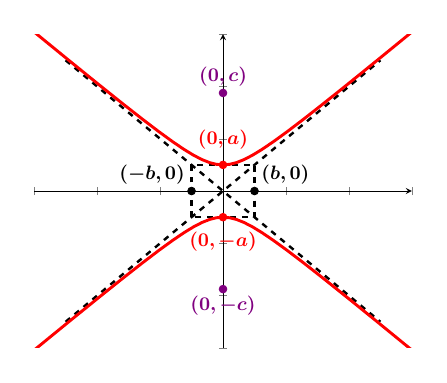
\begin{tikzpicture}[scale=0.7]
\begin{axis}[
axis lines = middle,
%grid,
xticklabels = {},
yticklabels = {},
xmin = -6, xmax = 6,
ymin = -6, ymax = 6
]
\draw [dashed, line width=1.25] (-1,-1) rectangle (1,1);
\draw [dashed, line width=1.25] (-5,-5) -- (5,5);
\draw [dashed, line width=1.25] (-5,5) -- (5,-5);
\addplot [red, line width = 1.5, domain=-2.5:2.5] ({sinh(x)}, {cosh(x)});
\addplot [red, line width = 1.5, domain=-2.5:2.5] ({sinh(x)}, {-cosh(x)});
\draw [fill=red, color=red] (0,1) circle (2pt);
\node at (0,1) [anchor=south, color=red, yshift=0.15cm] {$\bm{(0,a)}$};
\draw [fill=blue, color=red] (0,-1) circle (2pt);
\node at (0,-1) [anchor=north, color=red, yshift=-0.15cm] {$\bm{(0,-a)}$};
\draw [fill=violet, color=violet] (0,3.75) circle (2pt);
\node at (0,3.75) [anchor=south, color=violet] {$\bm{(0,c)}$};
\draw [fill=violet, color=violet] (0,-3.75) circle (2pt);
\node at (0,-3.75) [anchor=north, color=violet] {$\bm{(0,-c)}$};
\draw [fill=black] (1,0) circle (2pt);
\node at (1,0) [anchor=south west] {$\bm{(b,0)}$};
\draw [fill=black] (-1,0) circle (2pt);
\node at (-1,0) [anchor=south east] {$\bm{(-b,0)}$};
\end{axis}
\end{tikzpicture}   \newline\\
\begin{tabular}{rl}
    \onslide<2->{\textbf{\textit{x}-Axis}       &   Conjugate Axis}    \\[0.15in]
    \onslide<3->{\textbf{\textit{y}-Axis}       &   Traverse Axis}    \\
\end{tabular}
\end{center}
\end{frame}

\begin{frame}{Intro}
\begin{center}
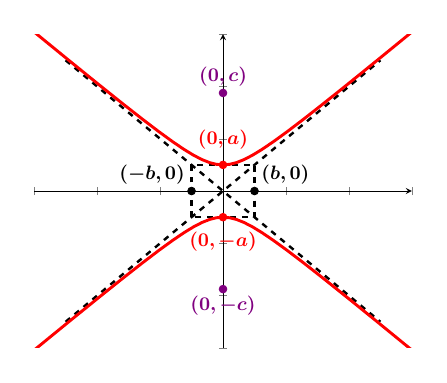
\begin{tikzpicture}[scale=0.7]
\begin{axis}[
axis lines = middle,
%grid,
xticklabels = {},
yticklabels = {},
xmin = -6, xmax = 6,
ymin = -6, ymax = 6
]
\draw [dashed, line width=1.25] (-1,-1) rectangle (1,1);
\draw [dashed, line width=1.25] (-5,-5) -- (5,5);
\draw [dashed, line width=1.25] (-5,5) -- (5,-5);
\addplot [red, line width = 1.5, domain=-2.5:2.5] ({sinh(x)}, {cosh(x)});
\addplot [red, line width = 1.5, domain=-2.5:2.5] ({sinh(x)}, {-cosh(x)});
\draw [fill=red, color=red] (0,1) circle (2pt);
\node at (0,1) [anchor=south, color=red, yshift=0.15cm] {$\bm{(0,a)}$};
\draw [fill=blue, color=red] (0,-1) circle (2pt);
\node at (0,-1) [anchor=north, color=red, yshift=-0.15cm] {$\bm{(0,-a)}$};
\draw [fill=violet, color=violet] (0,3.75) circle (2pt);
\node at (0,3.75) [anchor=south, color=violet] {$\bm{(0,c)}$};
\draw [fill=violet, color=violet] (0,-3.75) circle (2pt);
\node at (0,-3.75) [anchor=north, color=violet] {$\bm{(0,-c)}$};
\draw [fill=black] (1,0) circle (2pt);
\node at (1,0) [anchor=south west] {$\bm{(b,0)}$};
\draw [fill=black] (-1,0) circle (2pt);
\node at (-1,0) [anchor=south east] {$\bm{(-b,0)}$};
\end{axis}
\end{tikzpicture}   \newline\\
\begin{tabular}{rl}
    \onslide<2->{$\bm{c^2}$     &   $=a^2+b^2$ }  \\[0.15in]
    \onslide<3->{\textbf{Asymptotes}    &   $y = \pm\dfrac{a}{b}(x-h)+k$}  \\
\end{tabular}
\end{center}
\end{frame}


\section{Find the center, vertices, foci, and asymptote equations for a hyperbola.}

\begin{frame}{Example 1}
Find the center, vertices, foci, and equations of the asymptotes for the hyperbola \[\frac{(x-2)^2}{4} - \frac{y^2}{25} = 1\]  
\begin{minipage}{0.5\textwidth}
\onslide<2->{
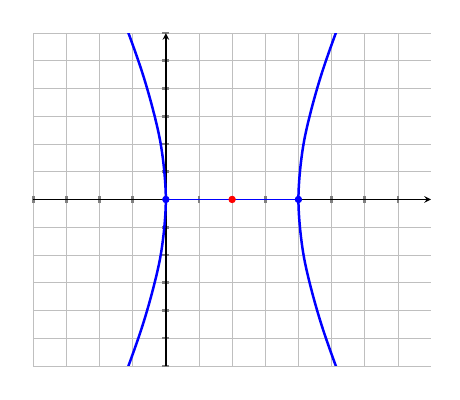
\begin{tikzpicture}[scale=0.6]
\begin{axis}[
axis lines = middle,
axis line style = thick,
tick style = ultra thick,
grid,
xtick = {-4,-3,...,7},
ytick = {-6,-5,...,6},
xticklabels = {},
yticklabels = {},
xmin = -4, xmax = 8,
ymin = -6, ymax = 6,
width = 10cm,
]
\addplot [blue, line width = 1.5, domain=-5:5, smooth] ({2*cosh(x)+2}, {5*sinh(x)});
\addplot [blue, line width = 1.5, domain=-5:5, smooth] ({-2*cosh(x)+2}, {5*sinh(x)});
\addplot [mark=*, color=red] coordinates { (2,0) };
\addplot [mark=*, color=blue] coordinates {(0,0) (4,0)};
\end{axis}
\end{tikzpicture}}
\end{minipage}
\hspace{0.25cm}
\begin{minipage}{0.45\textwidth}
\onslide<3->{{\color{red}Center: $(2, 0)$}   \\[8pt]} 
\onslide<4->{$a^2 = 4 \longrightarrow a = \pm 2$} \\[8pt]
\onslide<5->{{\color{blue}Vertices: $(2 \pm 2, 0)$}} \\[8pt]
\onslide<6->{{\color{blue}Vertices: $(0,0)$ and $(4,0)$}} \\[8pt]
\end{minipage}
\end{frame}

\begin{frame}{Example 1 $\frac{(x-2)^2}{4} - \frac{y^2}{25} = 1$}
\begin{minipage}{0.5\textwidth}
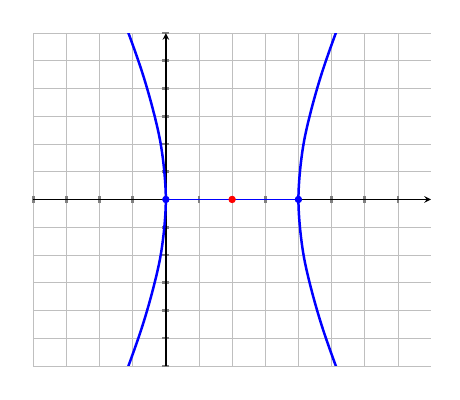
\begin{tikzpicture}[scale=0.6]
\begin{axis}[
axis lines = middle,
axis line style = thick,
tick style = ultra thick,
grid,
xtick = {-4,-3,...,7},
ytick = {-6,-5,...,6},
xticklabels = {},
yticklabels = {},
xmin = -4, xmax = 8,
ymin = -6, ymax = 6,
width = 10cm,
]
\addplot [blue, line width = 1.5, domain=-5:5, smooth] ({2*cosh(x)+2}, {5*sinh(x)});
\addplot [blue, line width = 1.5, domain=-5:5, smooth] ({-2*cosh(x)+2}, {5*sinh(x)});
\addplot [mark=*, color=red] coordinates { (2,0) };
\addplot [mark=*, color=blue] coordinates {(0,0) (4,0)};
\end{axis}
\end{tikzpicture}
\end{minipage}
\hspace{0.25cm}
\begin{minipage}{0.45\textwidth}
\onslide<2->{{\color{violet}Foci: $c^2 = a^2 + b^2$}} \\[8pt]
\onslide<3->{{\color{violet}Foci: $c^2 = 4 + 25$}} \\[8pt]
\onslide<4->{{\color{violet}Foci: $c = \pm \sqrt{29}$}} \\[8pt]
\onslide<5->{{\color{violet}Foci: $(2 \pm \sqrt{29}, 0)$}} \\[8pt]
\end{minipage}
\end{frame}

\begin{frame}{Example 1}
\begin{center}
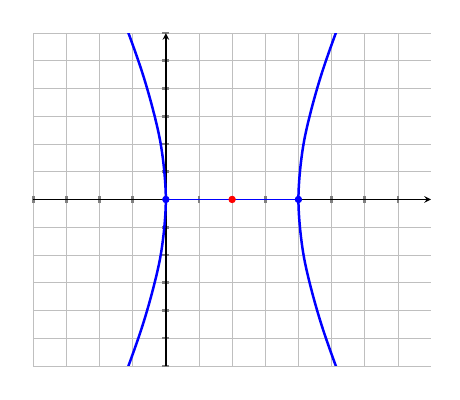
\begin{tikzpicture}[scale=0.6]
\begin{axis}[
axis lines = middle,
axis line style = thick,
tick style = ultra thick,
grid,
xtick = {-4,-3,...,7},
ytick = {-6,-5,...,6},
xticklabels = {},
yticklabels = {},
xmin = -4, xmax = 8,
ymin = -6, ymax = 6,
width = 10cm,
]
\addplot [blue, line width = 1.5, domain=-5:5, smooth] ({2*cosh(x)+2}, {5*sinh(x)});
\addplot [blue, line width = 1.5, domain=-5:5, smooth] ({-2*cosh(x)+2}, {5*sinh(x)});
\addplot [mark=*, color=red] coordinates { (2,0) };
\addplot [mark=*, color=blue] coordinates {(0,0) (4,0)};
\end{axis}
\end{tikzpicture}   \newline\\
\onslide<2->{Asymptotes: $y - 0 = \pm \frac{5}{2}(x-2)$}    \\[8pt]
\onslide<3->{Asymptotes: $y = \pm \frac{5}{2}(x-2)$} \\[8pt]
\onslide<4->{$y = \frac{5}{2}x-5$ and $y = -\frac{5}{2}x+5$}
\end{center}
\end{frame}

\section{Write the equation for a hyperbola in standard form.}

\begin{frame}{Writing Equations in Standard Form}
Writing the equation of a hyperbola in standard form uses a similar approach to that for ellipses. \emph{However, the negative term will actually be \underline{subtracted} from the right side.}    \newline\\
\end{frame}

\begin{frame}{Example 2a}
Find the center, vertices, foci, and equations of the asymptotes for each hyperbola. \newline\\
(a) \quad $9x^2+162x-16y^2+64y+89=0$
\begin{align*}
    \onslide<2->{{\color{red}9x^2+162x}{\color{blue}-16y^2+64y} &= -89} \\[8pt]
    \onslide<3->{{\color{red}\text{Vertex: }(-9,-729)} \quad & \quad {\color{blue}\text{Vertex: }(2, 64)}} \\[8pt]
    \onslide<4->{9(x+9)^2 - 16(y-2)^2 &= -89 + |{\color{red}-729}| - |{\color{blue}64}|} \\[8pt]
    \onslide<5->{9(x+9)^2 - 16(y-2)^2 &= 576} \\[8pt]
    \onslide<6->{\frac{(x+9)^2}{64} - \frac{(y-2)^2}{36} &= 1} \\
\end{align*}
\end{frame}

\begin{frame}{Example 2a}
\begin{center}
    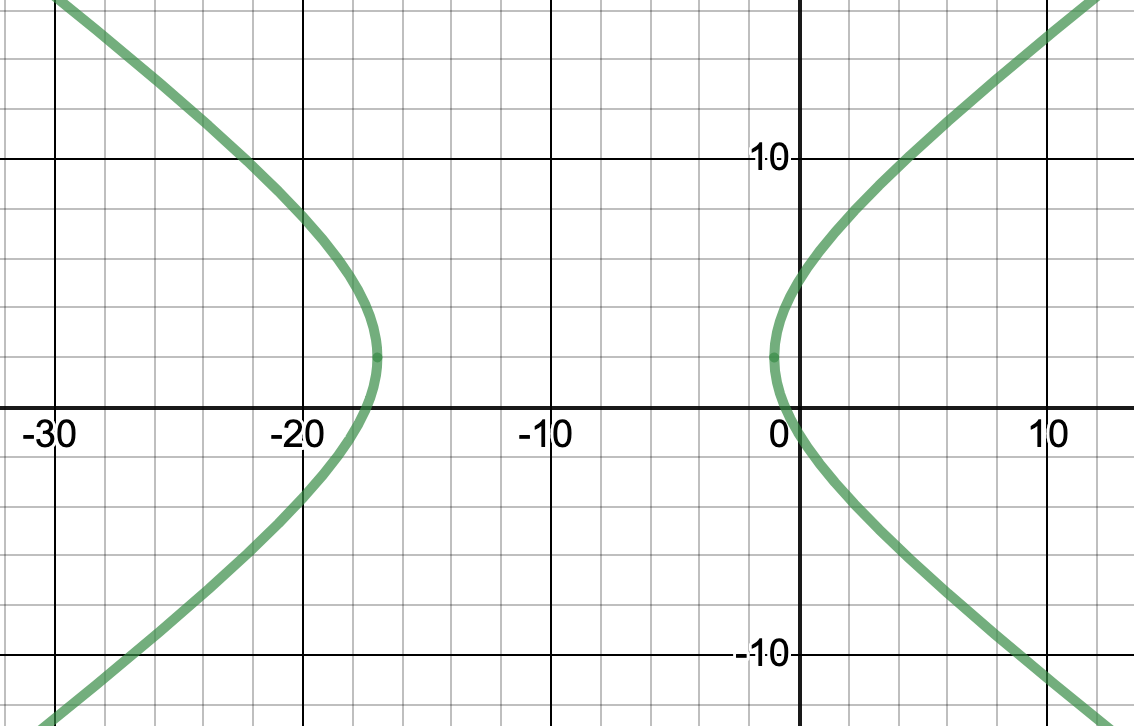
\includegraphics[scale=0.5]{ex2a.png}
\end{center}
\end{frame}

\begin{frame}{Example 2a \quad $\frac{(x+9)^2}{64} - \frac{(y-2)^2}{36} = 1$}
    \begin{align*}
        \text{Center: } & (-9,2) \\[8pt]
        \onslide<2->{a^2 &= 64} \\[8pt]
        \onslide<3->{a &= \pm 8} \\[8pt]
        \onslide<4->{\text{Vertices: } & (-9 \pm 8, 2)} \\[8pt]
        \onslide<5->{\text{Vertices: } & (-17,2) \text{ and } (-1,2)} \\[8pt]
    \end{align*}
\end{frame}

\begin{frame}{Example 2a \quad $\frac{(x+9)^2}{64} - \frac{(y-2)^2}{36} = 1$}
    \begin{align*}
        c^2 &= 64 + 36 \\[8pt]
        \onslide<2->{c &= \sqrt{100} = 10} \\[8pt]
        \onslide<3->{\text{Foci: } & (-9 \pm 10, 2)}\\[8pt]
        \onslide<4->{\text{Foci: } & (-19,2) \text{ and } (1,2)} \\
    \end{align*}
\end{frame}

\begin{frame}{Example 2a \quad $\frac{(x+9)^2}{64} - \frac{(y-2)^2}{36} = 1$}
    $a = 8 \quad b = 6 \quad \text{Center: }(-9,2)$
    \begin{align*}
        y &= \pm \frac{6}{8}(x+9) + 2 \\[8pt]
        y &= \pm \frac{3}{4}(x+9) + 2 
    \end{align*}
\end{frame}


\begin{frame}{Example 2b}
Find the center, vertices, foci, and equations of the asymptotes for each hyperbola. \newline\\
(a) \quad $9y^2 - x^2 - 6x = 10$
\begin{align*}
    \onslide<2->{{\color{blue}9y^2} {\color{red}-1x^2-6x} &= 10} \\[8pt]
    \onslide<3->{{\color{blue}\text{Vertex: }(0,0)} \quad & \quad {\color{red}\text{Vertex: }(-3,9)}} \\[8pt]
    \onslide<4->{9(y-0)^2 - (x+3)^2 &= 10 + |{\color{blue}0}| - |{\color{red}9}|} \\[8pt]
    \onslide<5->{9(y-0)^2 - (x-3)^2 &= 1} \\[10pt]
    \onslide<6->{\frac{(y-0)^2}{\frac{1}{9}} - \frac{(x-3)^2}{1} &= 1} \\
\end{align*}
\end{frame}

\begin{frame}{Example 2b}
    \begin{center}
        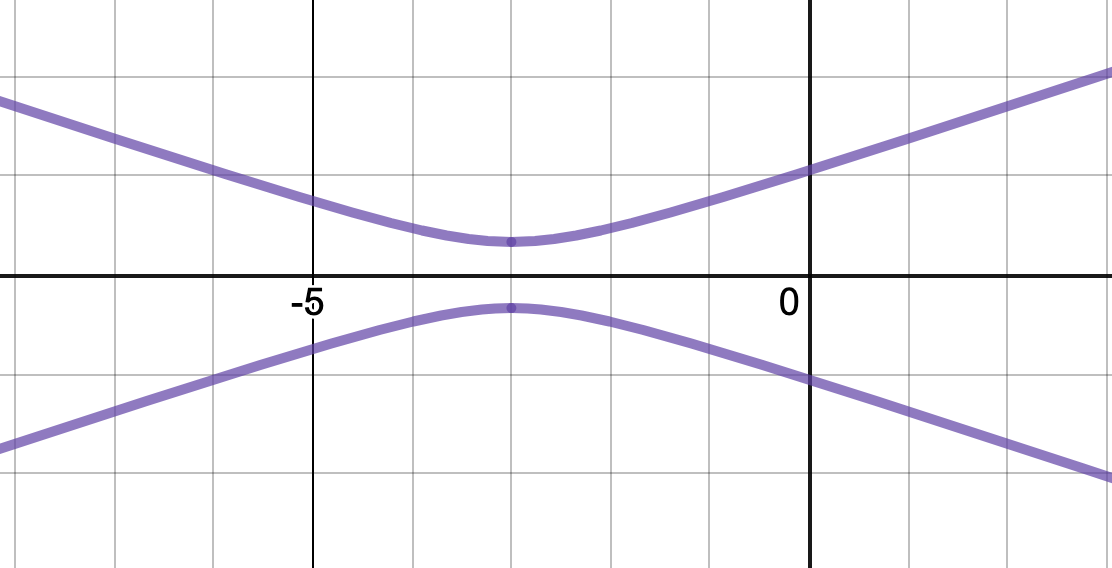
\includegraphics[scale=0.5]{ex2b.png}
    \end{center}
\end{frame}

\begin{frame}{Example 2b \quad $\frac{(y-0)^2}{\frac{1}{9}} - \frac{(x-3)^2}{1} = 1$}
    \begin{align*}
      \text{Center: } & (3,0) \\[8pt]
      \onslide<2->{a^2 &= \frac{1}{9}} \\[8pt]
      \onslide<3->{a &= \frac{1}{3}} \\[8pt]
      \onslide<4->{\text{Vertices: } & \left(3, 0\pm \frac{1}{3}\right)}  \\[8pt]
      \onslide<5->{\text{Vertices: } & \left(3, \pm \frac{1}{3}\right)} \\[8pt]
    \end{align*}
\end{frame}

\begin{frame}{Example 2b \quad $\frac{(y-0)^2}{\frac{1}{9}} - \frac{(x-3)^2}{1} = 1$}
    \begin{align*}
      c^2 &= \frac{1}{9} + 1 \\[8pt]
      \onslide<2->{c^2 &= \frac{10}{9}} \\[10pt]
      \onslide<3->{c &= \frac{\sqrt{10}}{3}} \\[10pt]
      \onslide<4->{\text{Foci: } & \left(3, \frac{1}{3} \pm \frac{\sqrt{10}}{3}\right)} \\[10pt]
      \onslide<5->{\text{Foci: } & \left(3, \frac{1 \pm \sqrt{10}}{3}\right)} \\
    \end{align*}
\end{frame}

\begin{frame}{Example 2b \quad $\frac{(y-0)^2}{\frac{1}{9}} - \frac{(x-3)^2}{1} = 1$}
\[
a = \frac{1}{3} \quad b = 1 \quad \text{Center: }(3,0)
\]
    \begin{align*}
    \onslide<2->{y &= \pm \frac{1/3}{1}(x-3) - 0} \\[8pt]
    \onslide<3->{y &= \pm \frac{1}{3}(x-3)} \\
    \end{align*}
\end{frame}


\begin{frame}{Example 3}
Find the equation of the hyperbola with asymptotes $y = \pm 2x$ and vertices $(\pm 5, 0)$.  \newline\\
\begin{minipage}{0.5\textwidth}
\onslide<2->{
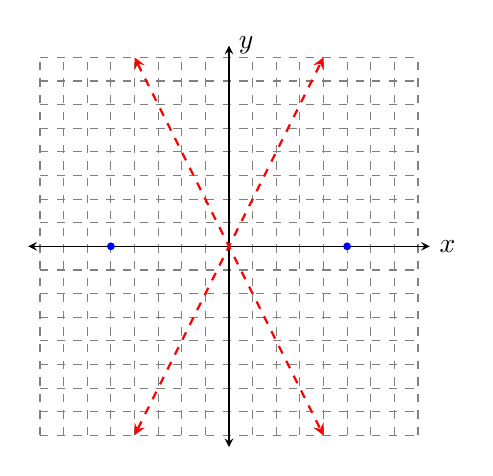
\begin{tikzpicture}[scale=0.3]
    \draw [dashed,gray] (-8,-8) grid (8,8);
    \draw[<->,>=stealth] (-8.5,0) -- (8.5,0) node [right] {$x$};
    \draw[<->,>=stealth] (0,-8.5) -- (0,8.5) node [right] {$y$};
    \draw[dashed,<->,>=stealth, thick, red] (-4,8) -- (4,-8);
    \draw[dashed,<->,>=stealth, thick, red] (-4,-8) -- (4,8);
    \draw[color=blue,fill=blue] (-5,0) circle (4pt);
    \draw[color=blue,fill=blue] (5,0) circle (4pt);
\end{tikzpicture}}
\end{minipage}
\hspace{0.25cm}
\begin{minipage}{0.4\textwidth}
\begin{align*}
    \onslide<3->{\color{blue} a &= 5} \\[8pt]
    \onslide<4->{\frac{b}{5} &= 2} \\[8pt]
    \onslide<5->{b &= 10} \\[8pt]
    \onslide<6->{\frac{x^2}{25} - \frac{y^2}{100} &= 1} \\
\end{align*}
\end{minipage}
\end{frame}

\end{document}
